\section{Conceitos básicos}

  Algumas definições são importantes para o bom entendimento do trabalho, sob pena de estabelecer ambiguidades ou equívocos quanto ao que se deseja propor. Sendo assim, no contexto deste trabalho, o que são testes e o que é desenvolvimento guiado por testes? o que é arquitetura de software e o que é uma arquitetura limpa? como desenvolvimento guiado por testes auxilia na obtenção de uma arquitetura limpa?

  \subsection{Testes}

    Se estabelecermos um marco na história da programação como sendo a parceiria entre a matemática londrina Ada Lovelace, e o, também, matemático londrino Charles Babbage \cite{Huskey1980}, pode-se dizer que essa disciplina possui mais de 180 anos, e com ela dois grande problemas: 1. especificar o comportamento de um software; 2. garantir que um software não possua defeitos.

    No primeiro, por mais avanços que se tenha feito no campo da engenharia de software, essa é, ainda, uma área bastante desafiadora. No último, Disjkstra estatuiu que \emph{testes mostram a presença, não a ausência de defeitos} \cite[pág. 16]{Nato1969}.

    Daí a necessidade de se testar \cite[pág. xxix-xxx]{Mezaros2007}: 1. paulatinamente construir conhecimento através da retroalimentação de hipóteses; 2. exaustivamente chegar a um ponto onde não é possível provar a presença de defeitos.

    Testes, segundo os métodos tradicionais de desenvolvimento, são feitos em etapa posterior a sua construção, para \emph{medir qualidade}. Uma abordagem diferente daquela que deseja \emph{construir qualidade} \cite[pág. 7]{FarcicGarcia2015}. Isso reverbera de maneira distinta \emph{quem} os executa: uma equipe independente daquela que construiu o software ou o próprio desenvolvedor?

  \subsection{Desenvolvimento guiado por testes}

    Dentre as práticas que sustentam os métodos ágeis, o uso de testes, como uma atividade de suporte às demais, é um fato consolidado. Mas a abordagem do TDD, também conhecida por \emph{testar primeiro} é ainda mais difundida nesse  meio.

    É bem corriqueiro ver profissionais se referindo à  técnica como "desenvolvimento orientado \emph{a} testes", dando a entender que seu objetivo é produzir um código que seja testável, o que é, claramente, uma consequência do seu uso. Ao passo que uma tradução que melhor exprime o conceito é "desenvolvimento orientado {por} testes".

    A ideia é extremamente simples \cite[p.1]{FreemanPryce2009}: \emph{escrever um teste para um código que ainda não existente}, sumariamente falando, mas de maneira mais completa, trata-se de um ciclo de três etapas \cite[pág. x]{Beck2003} - \figref{ciclo-tdd}: vermelho,  escreva um teste para o qual não existe uma implementação, portanto, não deve estar passando nesse momento; verde, faça o mesmo passar, escrevendo o código da funcionalidade pretendida; refactore, remova duplicações e melhore a legibilidade.

    \imagem
      {scale=0.75}
      {Ciclo de tdd}
      {ciclo-tdd.png}
      {ciclo-tdd}
      {Próprio autor\footnotemark}
    \footnotetext{Baseado na imagem encontrada no blog da Knowledge21 \url{https://knowledge21.com.br/blog/qualidade-de-software-com-tdd-test-driven-development/}}

    Essa postura realoca o papel dos testes de uma atividade meramente focada em descobrir defeitos para uma posição centrada na experiência do usuário, ao \emph{orientar} a desenvolvedora no entendimento das reais necessidades dos primeiros, através de um processo dialético de construção de conhecimento \footnote{\citeonline[p.28]{Oliveira1992} sugere, ao analisar Vygotsky e o processo de formação de conceitos, que os últimos são construções culturais, internalizadas pelos indivíduos ao longo do seu processo de desenvolvimento.}.

    Isso explica porque \citeonline[p.3-5]{FreemanPryce2009} colocam a prática como fundamentada em três pilares: 1. aprendizagem; 2. retroalimentação; e, 3. suporte a mudança.

  \subsection{Arquitetura de software}

    A engenharia de software, enquanto disciplina da ciência dos computadores, recebe o seu primeiro nome graças a uma série de propriedades que lhe são comuns com sua "aparentada" e seu sobrenome, em função de características que lhe são peculiares.

    Tal fenômeno, bastante comum nessa área do conhecimento, explica a denominação da chamada \emph{arquitetura de software} que, na ausência de uma expressão mais apropriada, toma emprestado a alcunha para conceituar uma abordagem com alto nível de abstração, que a "matéria dos dígitos binários" exige.

    Vejamos a definição do verbete inicial da locução: \emph{1. arte de projetar, construir, decorar e oraganizar os espaços de uma edificação; 2. obras arquitetônicas que caracterizam uma época ou povo} \cite[pág. 81]{Kury2007}.

    Ainda, etimologicamente, a palavra remete à composição grega de \emph{ARKHEIN} - que significa \emph{comandar}, em português - com \emph{TEKTON} - que, por sua vez, quer dizer \emph{artesão ou construtor}\footnote{Segundo o sítio "Etimologia - Origem do Conceito: Etimologia de Arquitetura". Disponível em: \url{https://etimologia.com.br/arquitetura/}. Acesso em: 6 de janeiro de 2021.}.

    Por aproximação, diz tratar-se dos dítames direcionadores de uma determinada construção. Ora, não resta dúvida, assim, que arquitetura de software são os preceitos orientadores de um sistema computacional.

  \subsection{Arquitetura limpa}

    Se ao vislumbrar determinada edificação é possível inferir algumas características de uma obra, seria possível realizar o mesmo exercício ao observar um "programa computacional"?

    A depender da forma como um prédio é arquitetado, é factível realizar alterações funcionais sem prejuízo à estrutura, ou, ainda, sem qualquer noção do dano que tais modificações podem desencadear.

    É esperado que a observação da plata baixa de uma edificação transmita informações suficientes para identificar do que se trata - uma casa, uma biblioteca, uma fábrica, etc. Essa é uma qualidade também desejável em um software, que alguns poucos artefatos sejam capazes de esclarecer o proprósito do mesmo. Ela deve \emph{gritar}.

  \citacaolonga
    {Então o que a arquitetura de sua aplicação grita? Quando você olha para o topo da sua estrutura de diretórios, e os arquivos fonte no pacote de mais alto nível, eles gritam "Sistema de Plano de Saúde," ou "Sistema de Contabilidade," ou "Sistema de Gerenciamento de Inventário"? Ou eles gritam "Rails," ou "Spring/Hibernate," ou "ASP"?}
    {\cite[pág. 196, tradução nossa]{Martin2018}}

  Muitos autores, ao longo de seus anos de experiência com desenvolvimento de software, estabeleceram suas próprias noções de arquitetura de sistemas, e apesar de terem nomes distintos - \emph{BCE}\cite{Jacobson1992}, \emph{Hexagonal}\cite{Cockburn2005}, \emph{Onion}\cite{Palermo2008}, \emph{DCI}\cite{Coplien2010} - elas compartilham características que as enquadram no conceito de \emph{Arquitetura Limpa}\cite{Martin2018}, notoriamente: \emph{Independente de frameworks}, \emph{Testável}, \emph{Independente de interface de usuário}, \emph{Independente de banco de dados} e {Independente de qualquer agente externo}.

  Elas também guardam a chamada \emph{Regra da Dependência}, onde, segundo \citeonline[p. 197, tradução nossa]{Martin2018} "as dependências do código fonte deve apontar somente na direção do centro do círculo, rumo as políticas de alto nível", como pode ser observado na \figref{clean-architecture}.

  \imagem
    {scale=0.4}
    {Modelo de Arquitetura Limpa}
    {CleanArchitecture.jpg}
    {clean-architecture}
    {\cite[pág. 197]{Martin2018}}

  \subsection{Como o desenvolvimento guiado por testes auxilia na obtenção de uma arquitetura limpa?}

    É fácil encontrar muitas similaridades entre a arquitetura convencional e a de software, mas existe um quesito que pesa a favor da última: como o nome sugere, soft (em português: flexível, suave) é um bem intangível, cuja construção, guardadas as devidas proporções e contextos, não oferece os mesmos riscos, por vezes irreparáveis, que a primeira está sujeita.

    Desenvolvimento guiado por testes privilegia uma conduta que permite definir as funções essenciais do sistema, implementá-las da maneira mais simplória conhecida e através de sucessivas modificações, amparadas por uma rede de proteção que previne regressões, alcançar um modelo que expressa, claramente, quais seus objetivos e permite uma evolução sustentável do produto.

\section{O estudo de caso}

  \subsection{O jogo}

    Hive\footnotemark é um jogo abstrato de duelo, tal qual o xadrez, onde os jogadores devem usar seus respectivos acervos para cercar o alvo oponente.
    \footnotetext{Tradução e adaptação nossa do sítio "UltraBoardGames: How to Play Hive". Disponível em: \url{https://www.ultraboardgames.com/hive/game-rules.php}. Acesso em: 29 de janeiro de 2021.}

    Cada jogador possui onze peças em formato hexagonal de cinco tipos distintos, cada tipo sendo representado por um inseto: uma abelha rainha, o alvo; duas aranhas; dois besouros; três gafanhotos; e, três formigas.

    Apenas uma ação, das duas possíveis, é permitida aos jogadores executar por turno: entrada e movimentação.

    Quando entra em jogo, uma peça deve ser colocada adjacente a uma que já está, à exceção daquela colocada no primiero turno do jogo. Ela também não deve tocar nenhuma peça adversária, reservada aquela que o faz no segundo turno, posto que a regra anterior deve ser atendida.

    A abelha rainha deve entrar, no máximo, até a quarta rodada. Enquanto isso não ocorrer, nenhuma peça irmã poderá ser movimentada.

    Os insetos tem movimentações diversas. A abelha rainha, um passo por vez ao redor da colméia. As aranhas, três passos ao redor da colméia, sempre na mesma direção iniciada. Os besouros, um passo ao redor da colméia ou acima dela, e a peça sob o qual ele pousa fica imobilizada até que ele a deixe e, para efeito de novas entradas, a posição ocupada assume a cor do mesmo. Os gafanhotos, se movimentam sobre a colméia, iniciando de um lado e seguindo em linha reta (perpendicular a aresta escolhida) até o lado oposto. E,  as formigas, o fazem ao redor da colméia sem limites de passos. Tais ações não podem resultar em uma colméia fragmentada, mesmo que o resultado seja uma colméia intacta. As movimentações ao redor devem ser de livre deslize, não sendo permitido entrar em uma posição onde isso não é possível.

    Finalmente, a abelha rainha é considerada cercada quando todos os seus lados estão ocupados por alguma peça em jogo, independente de a quem elas pertençam.

  \subsection{O escopo}

    O objetivo é construir uma aplicação onde um usuário qualquer possa se registrar para adquirir acesso. Uma vez autenticado ele pode propor ou responder a uma proposta de partida com um adversário que tenha realizado o mesmo caminho. E, obviamente, desempenhar uma partida. Deve, ainda, ser possível, organizar torneios, visualizar uma lista de classificação dos jogadores por suas respectivas pontuações e, apenas, observar uma partida, sem dela participar. É desejável que o registro e a autenticação possam ser realizados utilizando os mecanismos ofertados pelo Google e Facebook, bem como retomar uma partida que foi explicita ou implicitamente suspensa (um dos jogadores pode ter perdido a conexão por problemas em sua rede). Os jogadores devem ser capazes de convidar um adversário específico para uma partida. Também seria interessante que os usuários possam recuperar suas senhas que, ocasionalmente, possam vir a esquecer ou alterar informações sobre si (como nome que é apresentado aos demais, imagem de perfil, etc) além, é claro, de poder remover sua conta, caso não tenha mais interesse no serviço.

    Essa é uma descrição hipotética de necessidade inicial de um interessado em patrocinar um projeto dessa qualidade. Claro, em uma situação real, muitos outros detalhes deveriam ser capturados para refinar a solução, mas aqui vamos partir da premissa que esta é nossa única demanda.

  \subsection{A solução}

  Em função das limitações de tamanho e tempo, observou-se uma oportunidade para utilização de abordagem baseada em metodologias ágeis. No entanto, não é objetivo discorrer sobre o andamento de um projeto de software em sua completude mas, focar em algumas técnicas de desenvolvimento utilizadas. De tal forma, contamos com uma certa indulgência do leitor no que se refere a omissões descritivas dos caminhos gerenciais tomados.

  Usando \emph{histórias de usuário} como método de requisitos observamos a existência de muitas delas, de tal forma que se faz necessário organizar as mesmas dentro de um fluxo de capacidade mínimo \footnote{\citeonline{Patton2014} apresentam uma técnica, \emph{Mapeamento de Histórias de Usuário}, bastante útil para identificar fluxos e definir sua importância, em particular para o contexto em que não existe um proprietário de projeto - PO - capaz de priorizar as histórias que mais lhe agregam valor.} para completar as intenções firmadas no escopo. Daí se chega à \figref{mapeamento-historias-usuario}, onde se observa que 7 histórias são essenciais: \emph{criar conta; entrar; sair; chamar partida; atender chamado para partida; colocar peça em jogo; e, movimentar peça}. Isso define a abrangência do lançamento\footnote{Do inglês, \textbf{release}}. Sentimos, por experiência, que a última tem tendência para um \emph{épico}\footnote{\cite[pág. 6]{Cohn2004}}, por si só, mas,  para evitar a \emph{paralisia de análise}\footnote{\cite[pág. 71]{Pugh2011}}, vamos procrastinar a decisão de dividí-la\footnote{\cite[pág. 24]{Cohn2004}}, até que lidemos com ela especificamente. Esse sentimento também nos ajuda a escolher, para a primeira interação, a história de usuário \emph{Criar conta}.

  \imagem
    {width=16cm}
    {Mapeamento de histórias de usuário}
    {mapeamento-historias-de-usuario.miro}
    {mapeamento-historias-usuario}
    {Próprio autor\footnotemark}
  \footnotetext{Utilizando o serviço https://miro.com/}

  Factualmente, existem duas escolas de TDD: \emph{Chicago} - encontrada, ainda, como inside-out (de dentro para fora), classicista, bottom-up (de baixo para cima) - e \emph{Londres} - também conhecida como outside-in (de fora para dentro), mockista, top-down (de cima para baixo). Segundo \citeonline[págs. 488-492] {BryantPerez2019}, a tecnologia utilizada, mecanismos de construção, habilidades e preferências pessoais irão determinar que abordagem escolher. Mas também cita algumas características que ajudam nesta: possui bem delineadas as regras do negócio ou terá que traduzir o processo dos interessados em regras que possam ser automatizadas; existem restrições de plataforma (deve ser uma aplicação web, deve usar um determinado servidor de banco de dados, etc).

  Sendo assim, optamos pela abordagem londrina, que tem como principais representantes \citeonline{FreemanPryce2009}. A primeira observação é sobre o ciclo que, nessa perspectiva, possui dois níveis de execução (\figref{ciclo-atdd}). Graças a isso, é esperado que a etapa mais externa permanesça por mais tempo em estado de falha.

  \imagem
    {width=6cm}
    {Duplo ciclo da escola londrina de tdd}
    {ciclo-atdd}
    {ciclo-atdd}
    {Próprio autor\footnotemark}
  \footnotetext{Baseado na imagem encontrada em \citeonline[pág. 40]
  {FreemanPryce2009}}

  Também somos forçados a definir um esboço estrutural dos componentes (\figref{esboco-estrutural}) de auto nível sobre o qual repousaremos a solução (inicialmente - pois ela pode, ou não, vir a ser modificado durante o transcorrer do projeto).

  \imagem
    {width=6cm}
    {Esboço estrutural dos componentes da solução}
    {esboco-estrutural}
    {esboco-estrutural}
    {Próprio autor}

  Para levantar as histórias, \citeonline{Cohn2004} sugere o seguinte método: identificar os papéis; utilizá-los para construir narrativas no formato \emph{Connextra}\footnote{\citeonline{Connextra2001} propõs um modelo baseado na tríade \emph{papel-funcionalidade-benefício} ou, mais explicitamente, \narrativa{papel}{uma funcionalidade}{conseguir um benefício}}; levantar os critérios de aceite de cada história.

  Com a história \emph{Criar conta} chegamos a seguinte narrativa: \narrativa{visitante}{criar uma conta}{entrar e jogar uma partida}.

  Também foram levantados os seguintes critérios de aceite: deve ser informado um email válido; deve ser informada uma senha de tamanho mínimo 8 (oito) e tamanho máximo 20 (vinte) caracteres; não deve ser possível criar uma conta para um email que já vinculado a uma outra conta; deve constar um registro na base de dados.

  Já há elementos para elencarmos os cenários a serem trabalhados (\figref{criar-conta.cenarios}). Também é possível detalhar os passos de cada um deles usando o método sugerido por \citeonline{Nicieja2018} para derivação a partir dos critérios de aceite. O formato, \emph{Gherkin}, se baseia no artigo de \citeonline{North2006}.

  \imagem
    {width=10cm}
    {\textbf{Cenários} elencados para a \textbf{história} \emph{Criar conta}}
    {criar-conta.feature.png}
    {criar-conta.cenarios}
    {Próprio autor}

  Essa estrutura se alicerça na seguinte ideia: o passo identificado por \textbf{Dado} define o \emph{contexto} - pré-condição - onde a \emph{ação} (\textbf{Quando}) deve acontecer para que o \emph{resultado esperado} - pós-condição - (\textbf{Então}) seja observado.

  Há de salientar que os passos dos cenários descritos são, suficientemente, abstratos para permitir que os não-técnicos o leiam (ou, ainda, desejavelmente, os escrevam) mas não tanto que inviabilizar a sua automatização. Construímos o que \citeonline[pág. 24]{Evans2003} chama de \emph{linguagem ubíqua}. Dentre outros benefícios se pode citar a não fragilidade\footnote{\cite[pág. 93]{RoseWynneHellesoy2015} Do inglês, \textbf{brittle features}} desses artefatos, tornando-os resilientes às alterações de implementação, enquanto o comportamento esperado se mantiver intacto. Essa característica é essencial para subsidiar a \emph{refatoração}\footnote{\cite{Fowler1999}} e, por sua vez, é condição para o alvo mirado, a \emph{arquitetura limpa}.

  Retomando o esboço estrutural, o enriquecemos com os componentes que substituirão a figura humana no processo, dando vida própria a documentação\footnote{\citeonline[pág. 29]{Adzic2011} Live documentation}, donde se chega a \figref{esboco-estrutural-enriquecido}.

  \imagem
    {width=12cm}
    {Esboço estrutural enriquecido com os componentes que permitem a automatização}
    {esboco-estrutural-enriquecido}
    {esboco-estrutural-enriquecido}
    {Própio autor}

  Existem muitos mitos em torno das metodologias ágeis, e uma delas é a não existência de modelagem. Essa falsa crença se dá, muitas vezes, por uma noção equivocada de que documentação e modelos são equivalentes. \citeonline{Ambler2002} desconstrói esses mitos e mostra que essa atividade é, além de possível, basilar para um bom projeto de software. Isso nos permite, por exemplo, rabiscar uma solução para o cenário descrito\footnote{\citeonline[pág. 57]{Ruby2011} usa o mesmo processo para construir a solução apresentada no livro}, como pode ser observado na \figref{modelo-solucao.criar-conta-deve-ser-bem-sucedido.jpeg}.

  \imagem
    {width=12cm}
    {Modelo visual para solucionar o \textbf{cenário} \emph{deve ser bem sucedido} da \textbf{história} \emph{Criar conta}}
    {modelo-solucao.criar-conta-deve-ser-bem-sucedido.jpeg}
    {modelo-solucao.criar-conta-deve-ser-bem-sucedido.jpeg}
    {Própio autor}

  Esse ponto é auxiliado pelo que \citeonline[págs. 142 e 226]{Abelson1996} chama de \emph{wishful thinking}\footnote{Pensamento positivo, em tradução livre.} - mais precisamente o que \citeonline[pág. 45]{Astels2003} denomina \emph{programar por intenção} - para implementar os passos do cenário apresentados como se a funcionalidade pretendida já existisse. O objetivo é ser o mais claro possível sobre o que se almeja com aquela especificação, o resultado pode ser visto na \figref{criar-conta.deve-ser-bem-sucedido.passos}.

  \imagem
    {width=12cm}
    {Implementação dos passos do \textbf{cenário} \emph{deve ser bem sucedido} da \textbf{história} \emph{Criar conta}}
    {implementacao.cenario.js.png}
    {criar-conta.deve-ser-bem-sucedido.passos}
    {Própio autor}

  Essa etapa pode divergir bastante entre os diversos autores que tratam do tema, no que tange os conceitos de \emph{baby steps}\footnote{\cite[pág. 1]{Aniche2011}}, \emph{iniciar pelas verificações}, \emph{usar somente uma asserção por cenário}, \emph{não usar asserções fora da fase de verificação}. No fim, prevalecem, \emph{a familiaridade com as tecnologias empregadas}, \emph{a experiência no processo de desenvolvimento guiado por testes}, \emph{a simplicidade}\footnote{\cite[pág. xii]{Beck2003}}, mas, principalmente, \emph{o bom senso}.

  Como dito antes, o modelo londrino supõe a ciência prévia de determinados componentes da solução, de tal forma que o código da especificação funciona como uma tela de proteção no picadero de um circo funciona para os artistas do trapézio. Esse, talvez, seja o motivo de, algumas vezes, se tomar atalhos como o não uso de testes unitários em cenários em que, pela experiência, não apresentam grandes desafios. Ou seja, o desenvolvedor sabe o que quer fazer, mas para evitar horas procurando uma vírgula mal colocada, ele se utiliza da espeficifação automatizada para validar o caminho que ele está tomando. Essa mesma, lhe garantirá a não regressão de um caso, no momento em que um caminho mais elegante, internamente falando, for imaginado.

  Para este cenário, em particular, vemos, claramente, 2 componentes fundamentais: entrada de dados - ui (interface de usuário, mas poderia ser uma interface de código, se nossa solução fosse destinada a outros sistemas ao invés de humanos); e, saída de dados - db (que poderia envolver outros atores, como, por exemplo, um servidor de envio de mensagens eletrônicas externo, caso fossemos exigir ativação da conta por algum link encaminhado por email).

  Esperamos que, ao final da execução deste caso de teste, durante a verificação dos \emph{resultados esperados}, tenhamos um registro que nos comprove que a entrada de dados foi devidamente persistida. Isso deve ocorrer em contraposição ao \emph{contexto} do teste, em que o dito registro não deve existir. Assim nosso primeiro passo na direção da completude do cenário é a criação da consulta que faz a verificação da ausência do registro na base de dados (\figref{criar-conta-deve-ser-bem-sucedido-passo.dado}).

  \begin{figure}[h]
    \centering
    \caption{Implementação do código de suporte do cenário}
    \efbox{
      \makebox[\textwidth]{
        \begin{subfigure}[t]{0.5\textwidth}
          \centering
          \caption{Banco de dados}
          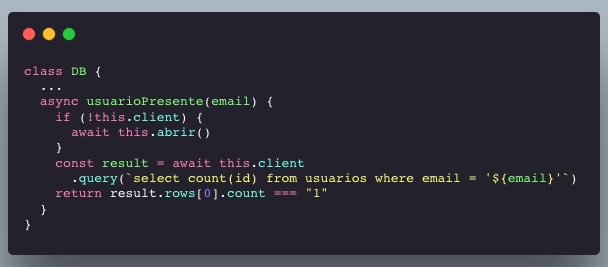
\includegraphics[width=\textwidth]{db.js.png}
          \label{fig:criar-conta-deve-ser-bem-sucedido-passo.dado}
          \label{fig:criar-conta-deve-ser-bem-sucedido-passo.entao}
        \end{subfigure}
        \hfill
        \begin{subfigure}[t]{0.5\textwidth}
          \centering
          \caption{Interface de usuário}
          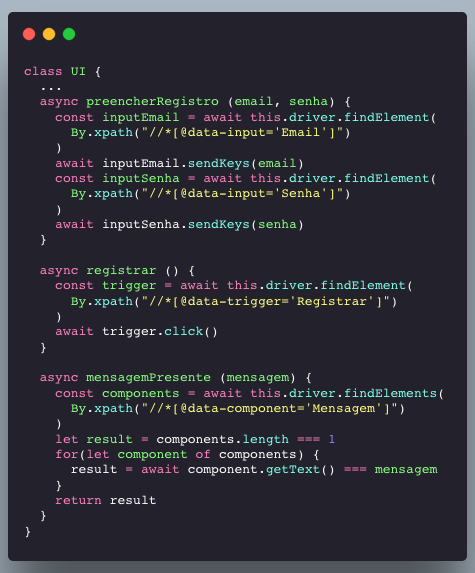
\includegraphics[width=\textwidth]{ui.js.png}
          \label{fig:criar-conta-deve-ser-bem-sucedido-passo.quando}
        \end{subfigure}
      }
    }
    Fonte: Próprio autor
    \label{fig:suporte-cenario}
  \end{figure}

  Para o passo que representa a ação, vemos que existem níveis de abstração, ao observar que o comando \emph{quando eu me registro}, na verdade é uma composição de 3 ações: abrir a página do formulário de registro; preencher os campos obrigatórios do mesmo (que, por si só, já é uma composição pois resume o preenchimento de muitos campos a uma única ação composta); e, finalmente, submeter essas informações pelo clique no botão \emph{registrar} (\figref{criar-conta-deve-ser-bem-sucedido-passo.quando}).

  Por fim, temos o passo de verificação, como já havíamos adiantado, reutilizamos o código de suporte da pré-condição que deve ter o efeito oposto nesse momento, bem como a da existência de uma mensagem de feedback do sucesso da ação (\figref{criar-conta-deve-ser-bem-sucedido-passo.entao}).

  Isso conclui o trabalho de construção da rede de proteção que nos permitirá implementar a funcionalidade com a confiança de que seremos apoiados pela especificação automatizada. Desse momento em diante, podemos, inclusive, escolher a plataforma que melhor nos convier (desde que atenda aos limites mínimos impostos, que nesse caso são: uma aplicação web e um banco de dados relacional suportado pela plataforma). Ou seja, a miriade de possibilidades em que essa solução pode ser implementada é enorme. Para o nosso caso, em particular, escolhemos um frontend em React e um backend em Java/Quarkus e um banco de dados PostgreSQL.

  Sem muito esforço chegamos a solução apresentada na \figref{primeira-solucao}.

  \begin{figure}[h]
    \centering
    \caption{Primeira versão da solução do cenário}
    \efbox{
      \makebox[\textwidth]{
        \begin{subfigure}[t]{0.25\textwidth}
          \centering
          \caption{Banco de dados}
          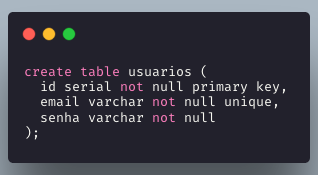
\includegraphics[width=\textwidth]{criar_usuarios.sql.png}
          \label{fig:banco de dados}
        \end{subfigure}
        \hfill
        \begin{subfigure}[t]{0.25\textwidth}
          \centering
          \caption{Frontend}
          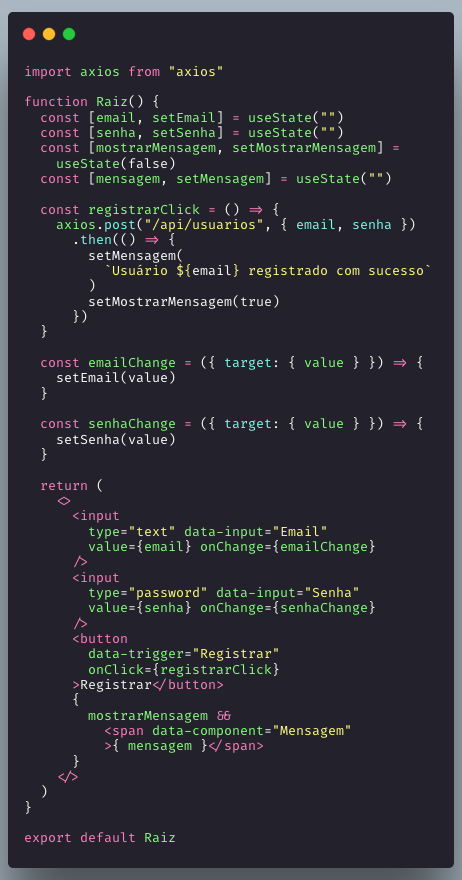
\includegraphics[width=\textwidth]{raiz.js.png}
          \label{fig:frontend}
        \end{subfigure}
        \linebreak
        \begin{subfigure}[t]{0.25\textwidth}
          \centering
          \caption{Backend: Main.java}
          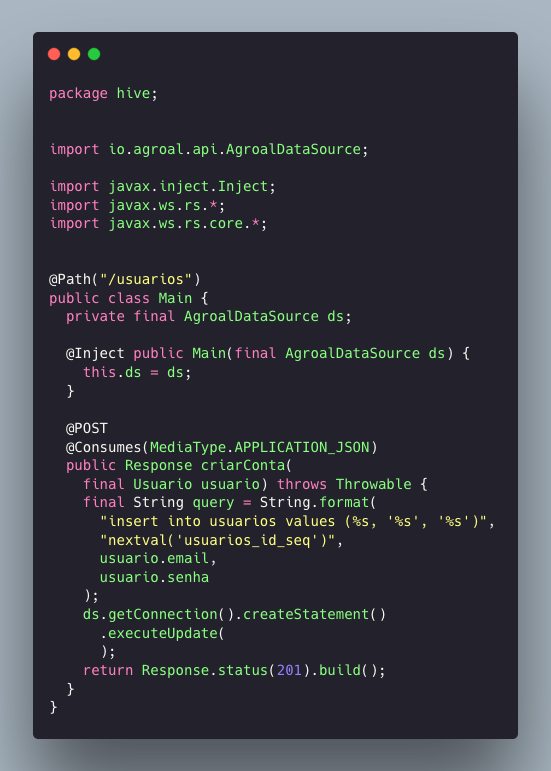
\includegraphics[width=\textwidth]{main.java.png}
          \label{fig:backend-main}
        \end{subfigure}
        \hfill
        \begin{subfigure}[t]{0.25\textwidth}
          \centering
          \caption{Backend: Usuario.java}
          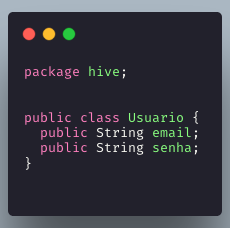
\includegraphics[width=\textwidth]{usuario.java.png}
          \label{fig:backend-usuario}
        \end{subfigure}
      }
    }
    Fonte: Próprio autor\footnote{Utilizando o serviço https://carbon.now.sh}
    \label{fig:primeira-solucao}
  \end{figure}

  Sigamos esse método para os demais cenários da \figref{criar-conta.cenarios}.

  Nesse momento, guardadas as devidas proporções, já se pode dizer que o valor imediato esperado pelo patrocinador foi entregue. No entanto, existe muito trabalho pela frente para tornar o produto atraente, muitas funcionalidades precisam ser incorporadas, e como se está utilizando metodologia ágeil, as decisões sobre as histórias de usuário vindouras são tomadas quando estas estiverem sob discussão. Ao contrário do que se costuma fazer em metodologias de desenvolvimento tradicionais, onde uma tentativa de premonição dos problemas a serem enfrentados é realizada, nesse caso é fundamental adotar práticas de desenho arquitetural que permitam extender as capacidades do sistema com o mínimo de trauma possível.

  Aqui entra em cena a atividade de refatoração. Ela permitirá alterar a estrutura interna do software sem que para isso se tenha que alterar o comportamento observável do mesmo. Isso só é possível porque existe uma rede de proteção chamada testes automatizados, que dirão se essa alteração maculou a forma como aquele foi especificado.

  É uma excelente oportunidade, ainda, para diminuir o débito técnico em torno das práticas de testes de unidade\footnote{Deixados de lado para fins didáticos, vez que a abordagem apresentada por \citeonline{FreemanPryce2009} prevê o uso dos mesmos como forma de exercitar a paulatina chegada à solução almejada.}. Também é possível observar que a utilização de testes dessa natureza, ao tempo que garantem um melhor projeto de código para software, não são suficientes para garantir que o mesmo de comporta como esperado - o famoso dilema \emph{fazer a coisa certa vs. fazer certo a coisa}\footnote{\emph{Doing things right} vs. \emph{Doing the right things}, segundo \citeonline{Poddar2018}, o primeiro diz sobre \emph{eficiência} enquanto o segundo se refere a \emph{efetividade}.}. Essa expressão leva a dedução de que os testes de aceitação e os testes de unidade são complementares, e negligenciar qualquer deles é um caminho para o insucesso de qualquer projeto.

  Isso leva a uma ponderação entre prós e contras sobre os tipos de testes. Se por um lado os testes de ponta a ponta permitem afirmar que as funcionalidade solicitadas foram entregues conforme as especificações, também é possível observar que quanto maior é a sua quantidade mais frustrantes é a experiência de utilizá-los como ferramenta de feedback, vez que seu tempo de execução é consideravelmente maior que a de testes de unidade.

  Para ser mais explícito, considere-se os cenários de exceção, da história de usuário em trabalho, onde se espera que os mesmo falhem por invalidade do email e da senha informados. É fácil perceber a necessidade de validar múltiplos valores e, provavelmente, o melhor lugar para fazê-lo não seja nos testes de funcionais, mas naqueles que não requerem acesso a recursos externos.

  Também se pode tirar proveito dessa abordagem para solidificar o entendimento do cerne do negócio (\figref{teste-de-unidade-caso-de-uso}) e abstrair as dependências que prestam serviços a ele.

  \begin{figure}[h]
    \centering
    \caption{Teste de unidade do caso de uso e respectiva solução}
    \efbox{
      \makebox[\textwidth]{
        \begin{subfigure}[t]{0.5\textwidth}
          \centering
          \caption{Teste de unidade}
          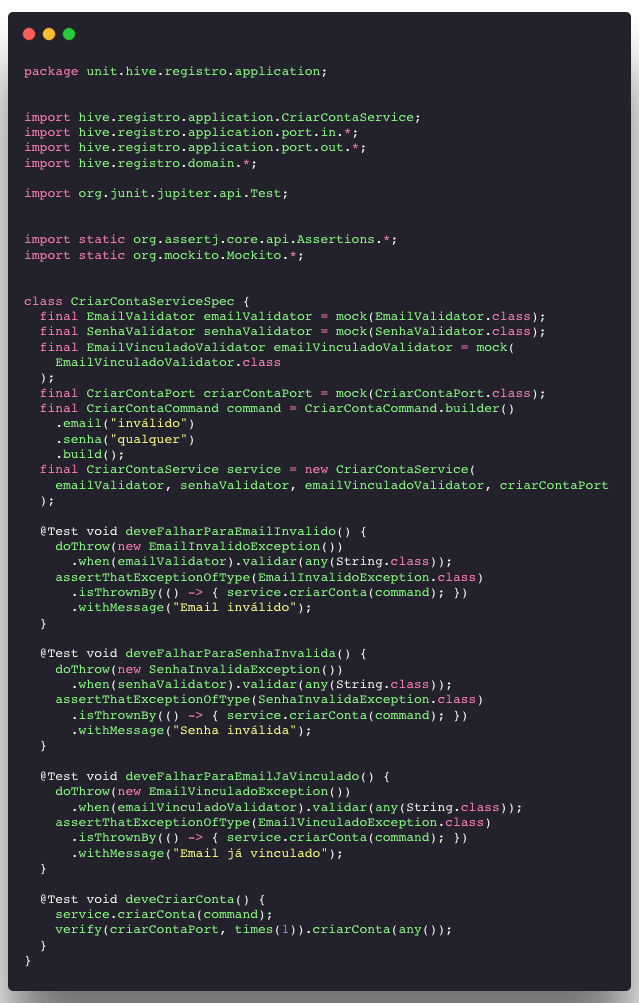
\includegraphics[width=\textwidth]{CriarContaServiceSpec.png}
          \label{fig:CriarContaServiceSpec}
        \end{subfigure}
        \hfill
        \begin{subfigure}[t]{0.5\textwidth}
          \centering
          \caption{Implementação do caso de uso}
          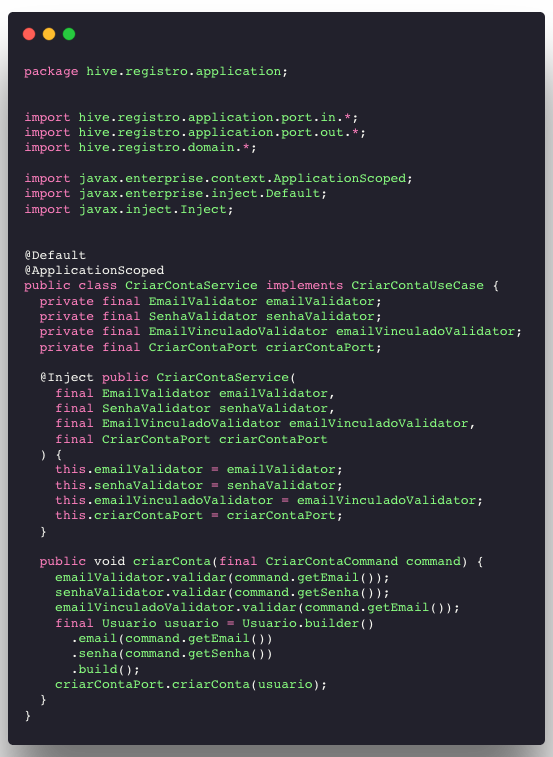
\includegraphics[width=\textwidth]{CriarContaService.png}
          \label{fig:CriarContaService}
        \end{subfigure}
      }
    }
    Fonte: Próprio autor
    \label{fig:teste-de-unidade-caso-de-uso}
  \end{figure}

  Isso capacita os testes isolados de funcionalidades de mais baixo nível (\figref{teste-de-unidade-email}), com o benefício de executarem de maneira celere, tendo como retaguarda os testes de mais alto nível para garantir que tais componentes se integram da forma esperada.

  \begin{figure}[h]
    \centering
    \caption{Teste de unidade de validação de email e respectiva solução}
    \efbox{
      \makebox[\textwidth]{
        \begin{subfigure}[t]{0.5\textwidth}
          \centering
          \caption{Teste de unidade}
          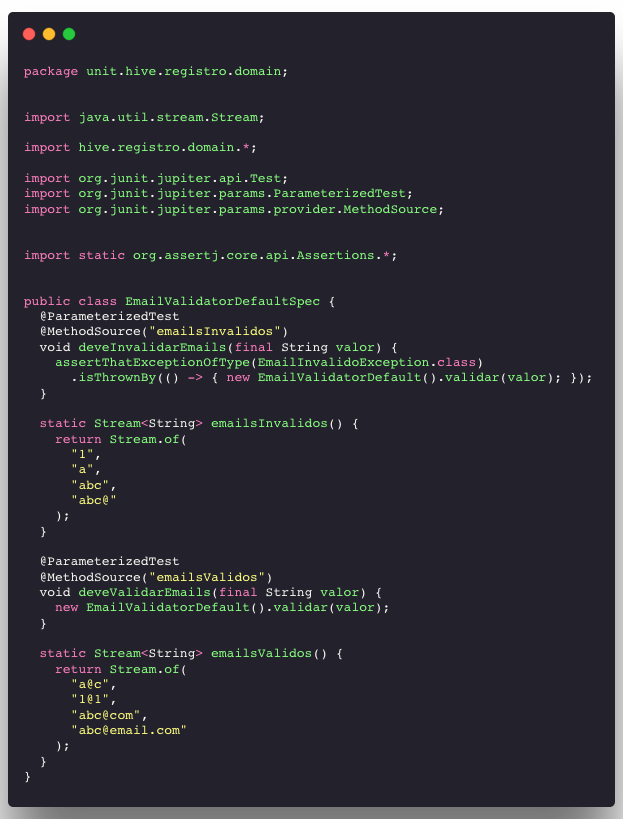
\includegraphics[width=\textwidth]{EmailValidatorDefaultSpec.png}
          \label{fig:EmailValidatorDefaultSpec}
        \end{subfigure}
        \hfill
        \begin{subfigure}[t]{0.5\textwidth}
          \centering
          \caption{Implementação da interface}
          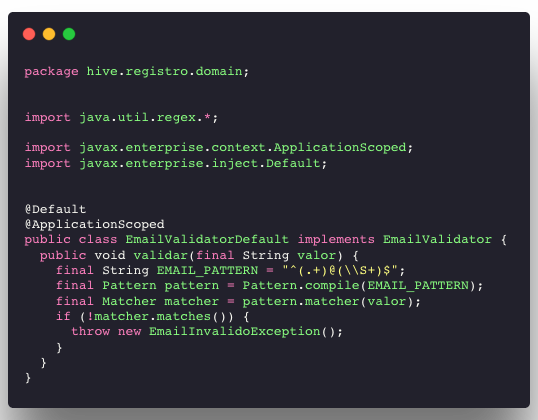
\includegraphics[width=\textwidth]{EmailValidatorDefault.png}
          \label{fig:EmailValidatorDefault}
        \end{subfigure}
      }
    }
    Fonte: Próprio autor
    \label{fig:teste-de-unidade-email}
  \end{figure}

	Esse método ainda permite focar a atenção sobre situações que podem ser difíceis de observar quando se verifica o conjunto de maneira holística (\figref{testes-de-integracao-api-e-repositorio}).

  \begin{figure}[h]
    \centering
    \caption{Teste de integração de api e repositório e respectiva solução}
    \efbox{
      \makebox[\textwidth]{
        \begin{subfigure}[t]{0.25\textwidth}
          \centering
          \caption{Teste de api}
          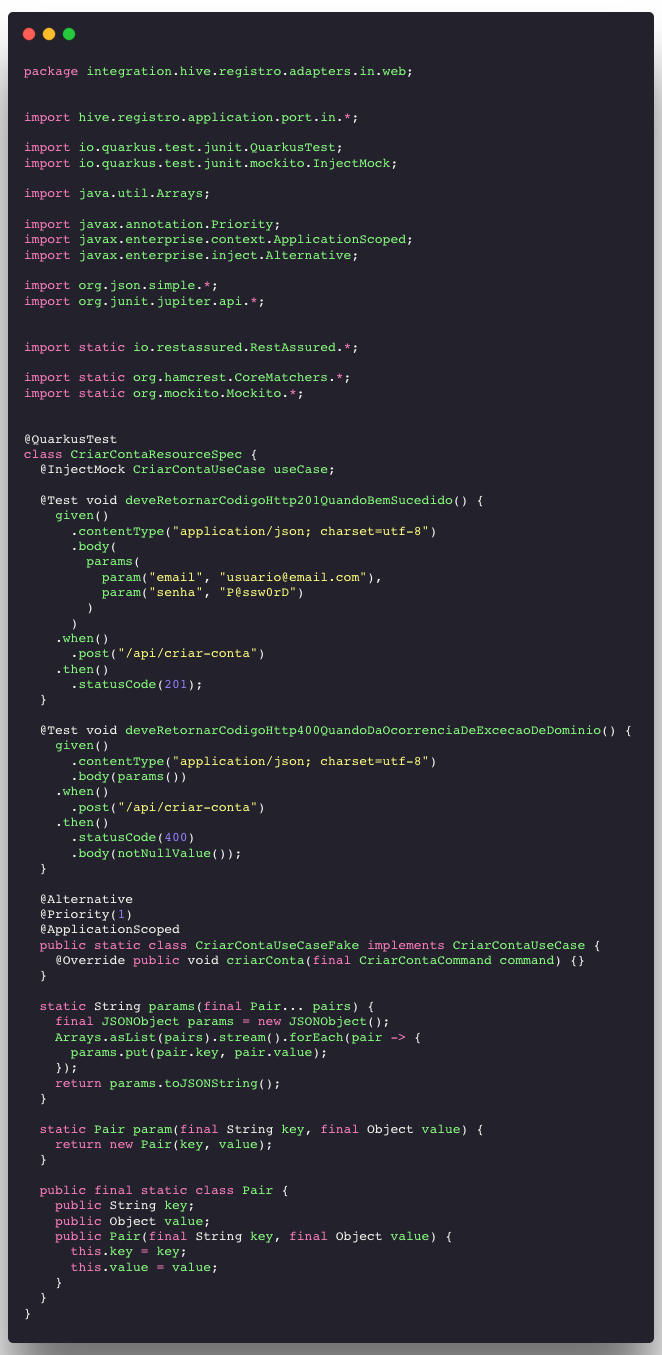
\includegraphics[width=\textwidth]{CriarContaResourceSpec.png}
          \label{fig:CriarContaResourceSpec}
        \end{subfigure}
        \hfill
        \begin{subfigure}[t]{0.25\textwidth}
          \centering
          \caption{Implementação da api}
          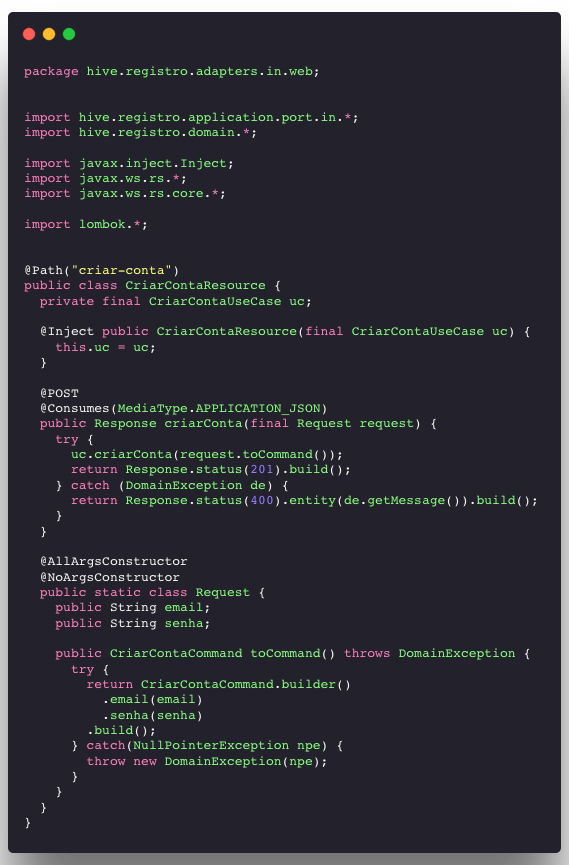
\includegraphics[width=\textwidth]{CriarContaResource.png}
          \label{fig:CriarContaResource}
        \end{subfigure}
        \hfill
        \begin{subfigure}[t]{0.25\textwidth}
          \centering
          \caption{Teste de repositório}
          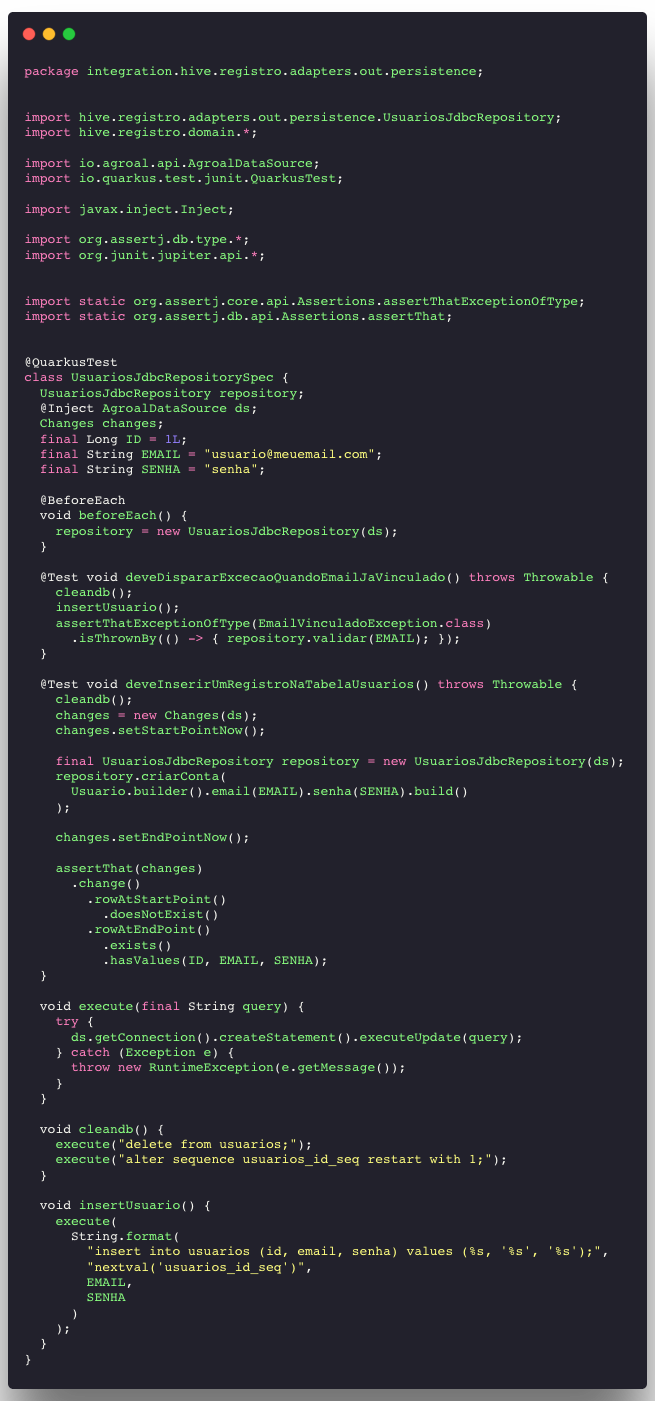
\includegraphics[width=\textwidth]{UsuariosJdbcRepositorySpec.png}
          \label{fig:UsuariosJdbcRepositorySpec}
        \end{subfigure}
        \hfill
        \begin{subfigure}[t]{0.25\textwidth}
          \centering
          \caption{Implementação de repositório}
          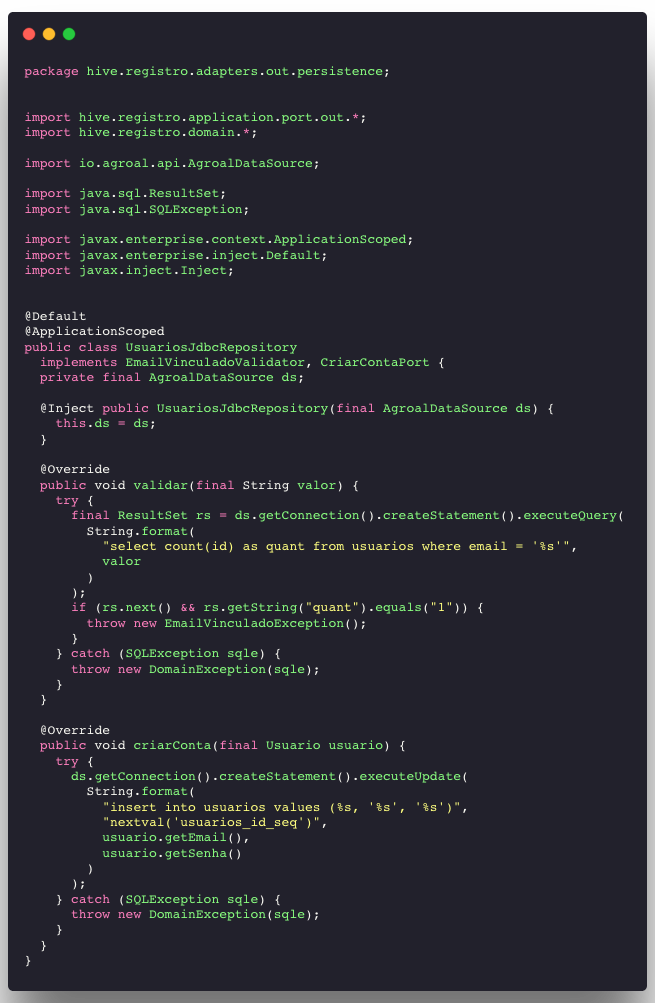
\includegraphics[width=\textwidth]{UsuariosJdbcRepository.png}
          \label{fig:UsuariosJdbcRepository}
        \end{subfigure}
      }
    }
    Fonte: Próprio autor
    \label{fig:testes-de-integracao-api-e-repositorio}
  \end{figure}

  A cobertura sobre a especificação é aumentada sem sacrificar o tempo de retroalimentação (Figura \textbf{testes de unidade da senha}).

  \begin{figure}[h]
    \centering
    \caption{Teste de unidade de validação de senha e respectiva solução}
    \efbox{
      \makebox[\textwidth]{
        \begin{subfigure}[t]{0.5\textwidth}
          \centering
          \caption{Teste de unidade}
          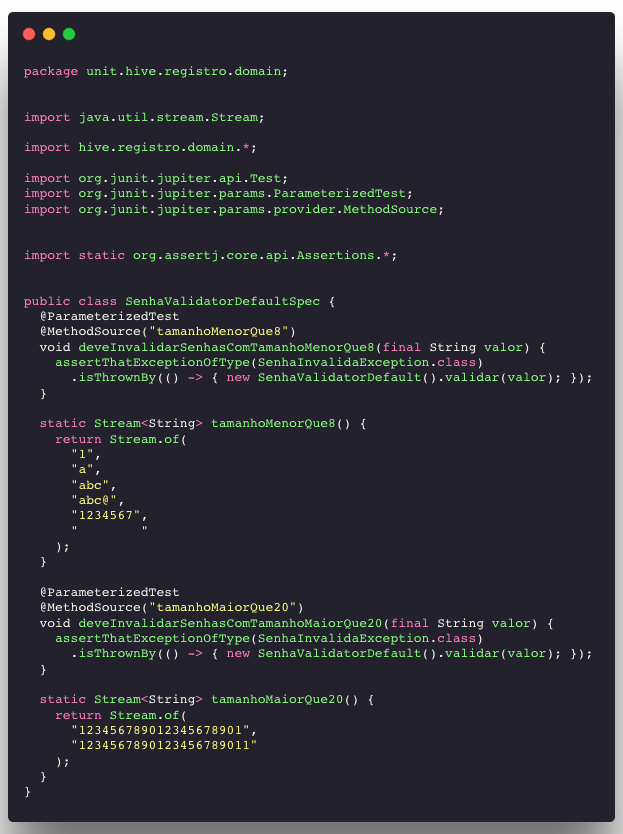
\includegraphics[width=\textwidth]{SenhaValidatorDefaultSpec.png}
          \label{fig:SenhaValidatorDefault}
        \end{subfigure}
        \hfill
        \begin{subfigure}[t]{0.5\textwidth}
          \centering
          \caption{Implementação do validador}
          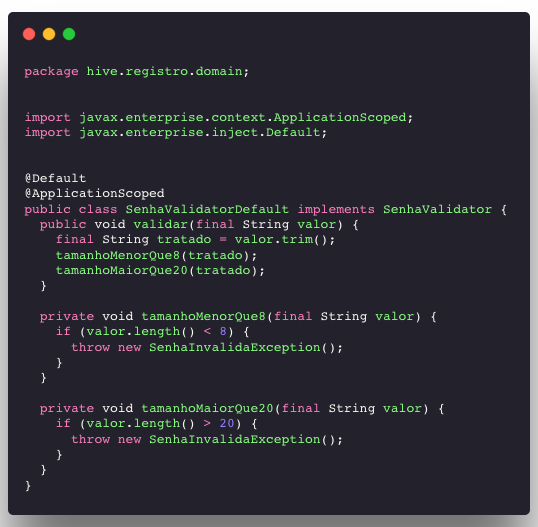
\includegraphics[width=\textwidth]{SenhaValidatorDefault.png}
          \label{fig:SenhaValidatorDefault}
        \end{subfigure}
      }
    }
    Fonte: Próprio autor
    \label{fig:testes-de-integracao-api-e-repositorio}
  \end{figure}

  Usando a proposta apresentada por \citeonline[pág. 21]{Hombergs2019}, se faz cumprir a meta de uma arquitetura que grita. Tal exigência é simples de ser visualizada pela árvora de pacotes (\figref{ArvoreBackend}).

  \begin{figure}[h]
    \centering
    \caption{Árvore de pacotes/diretórios do frontend e backend}
    \efbox{
      \makebox[\textwidth]{
        \begin{subfigure}[t]{0.5\textwidth}
          \centering
          \caption{Backend}
          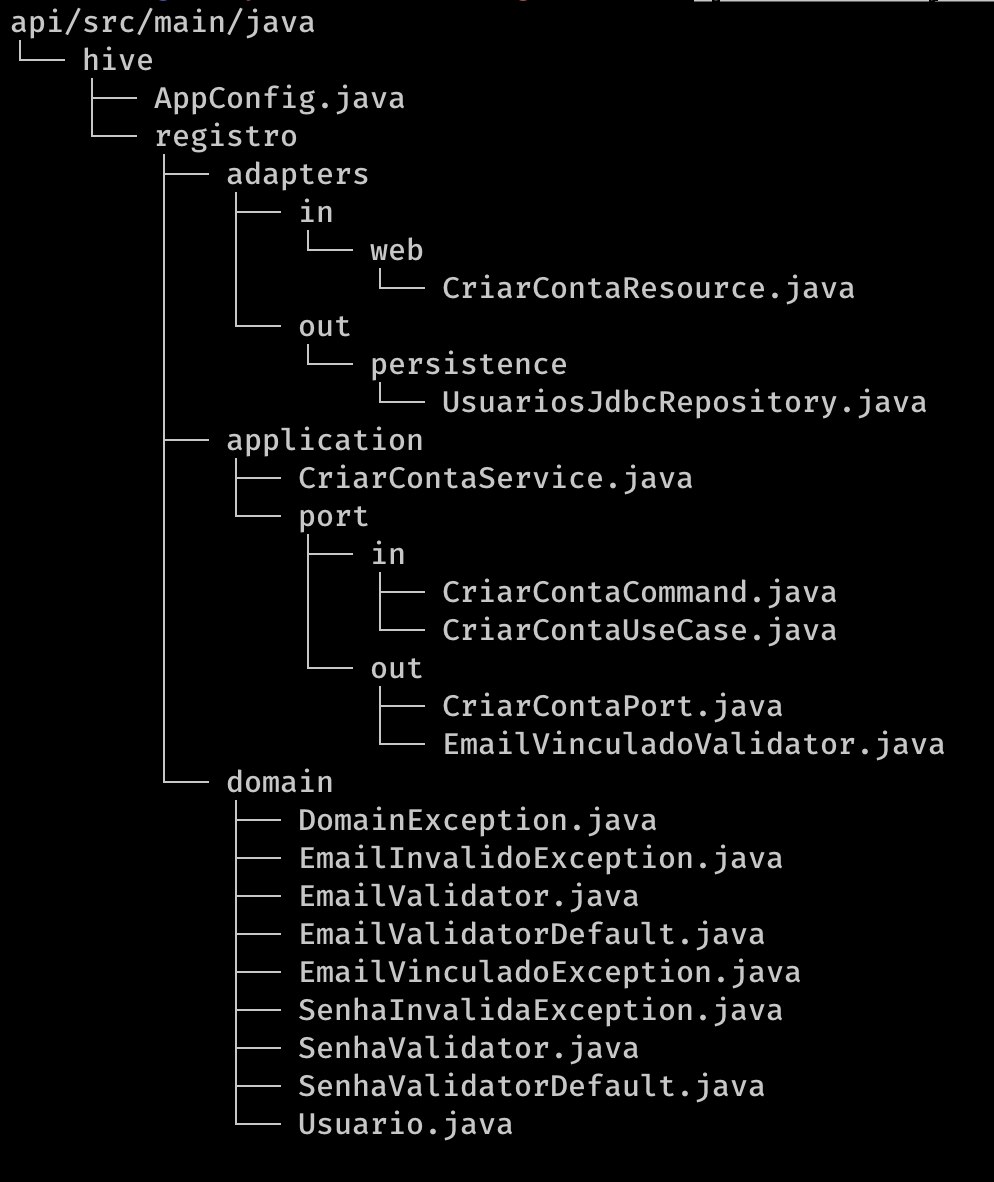
\includegraphics[width=\textwidth]{ArvoreBackend.png}
          \label{fig:ArvoreBackend}
        \end{subfigure}
        \hfill
        \begin{subfigure}[t]{0.5\textwidth}
          \centering
          \caption{Frontend}
          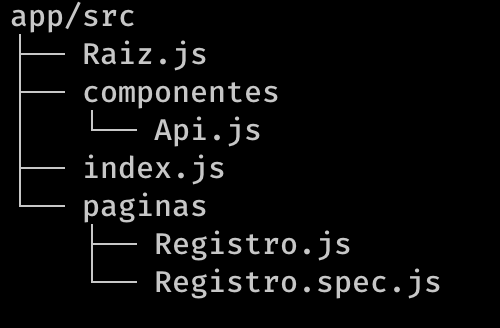
\includegraphics[width=\textwidth]{ArvoreFrontend.png}
          \label{fig:ArvoreFrontend}
        \end{subfigure}
      }
    }
    Fonte: Próprio autor
    \label{fig:testes-de-integracao-api-e-repositorio}
  \end{figure}

  Outro alvo da metodologia é a "lei" de referência das camadas, onde as mais externas conhecem as mais internas mas o contrário é uma violação arquitetural (\figref{clean-architecture}). De maneira geral, se pode constatar que os componentes do backend formam o desenho proposto por \citeonline{Cockburn2005}, que é uma arquitera limpa, conforme \citeonline[pág. 202]{Martin2018}.

  \imagem
    {width=5cm}
    {Modelo de arquitetura limpa}
    {CleanArchitecture.jpg}
    {clean-architecture}
    {The Clean Code Blog\footnotemark}
  \footnotetext{\cite{Martin2012}}

  Outra liberdade que se toma, nessa solução em particular, diz respeito a estruturação do código do frontend que, em não sendo uma parte da aplicação para o qual foi delegado muita responsabilidade, foi utilizada uma divisão baseada nas definições de \citeonline{Frost2016}, seja uma \emph{página}, do ponto de vista do usuário, sejam \emph{compoenentes}, que são integrados para formar aquelas (\figref{ArvoreFrontend}).

  Essa estrutura permite testar os componentes e páginas, novamente, de forma isolada (Figura \textbf{testes de unidade da página de registro}), ao passo que são resguardados pelos testes de aceitação.

